\subsection{Performance Evaluation}

Table \ref{tab:chap_6:benchmark} summarizes the evaluation results of our solution compared to competing TSC methods using various performance metrics, including accuracy, normalized accuracy, precision, recall, and F1-score. The results highlight the superiority of our approach over both one-stage and two-stage methods.


\begin{table*}[t]
\caption{Performance comparison on the datasets. Mean and standard deviation computed over five runs for Cloud VR datasets. Bold values indicate best results and underlined values the second best.}

\label{tab:chap_6:benchmark}
\setlength\tabcolsep{2pt}
\begin{tabular*}{\textwidth}{@{\extracolsep{\fill}}l | l | ccccc }
\toprule
\bf Models & \bf Metrics & \bf Accuracy & \bf N-Accuracy & \bf Precison & \bf Recall & \bf F1-score \\
\midrule
\multirow{4}{*}{\rotatebox{90}{\bf One-stage}} & 1-NN-DTW & 51.54$_{(\pm0.11)}$ & 26.36$_{(\pm0.17)}$ & 56.74$_{(\pm0.09)}$ & 51.54$_{(\pm0.11)}$ & 52.96$_{(\pm0.10)}$ \\
%& NN-DTW & $_{(\pm)}$ & $_{(\pm)}$ & $_{(\pm)}$ & $_{(\pm)}$ & $_{(\pm)}$ \\
\addlinespace
\cmidrule{2-7}
& T-Loss & \underline{79.47$_{(\pm4.39)}$} & \bf 75.22$_{(\bf\pm5.58)}$ & \bf 83.98$_{(\bf\pm4.74)}$ & \underline{79.47$_{(\pm4.39)}$} & \underline{79.60$_{(\pm4.53)}$} \\
\addlinespace
& TS2Vec & 70.12$_{(\pm5.28)}$ & 55.71$_{(\pm6.53)}$ & 75.42$_{(\pm3.22)}$ & 70.12$_{(\pm5.28)}$ & 70.49$_{(\pm4.88)}$ \\
\addlinespace
& TS-TCC & 73.78$_{(\pm6.38)}$ & 66.17$_{(\pm8.12)}$ & 79.29$_{(\pm6.07)}$ & 73.78$_{(\pm6.38)}$ & 73.86$_{(\pm6.68)}$ \\
\addlinespace
%& NN-DTW & $_{(\pm)}$ & $_{(\pm)}$ & $_{(\pm)}$ & $_{(\pm)}$ & $_{(\pm)}$ \\

\addlinespace
\midrule

\multirow{4}{*}{\rotatebox{90}{\bf Two-stage}} & iForest & 72.48$_{(\pm2.69)}$ & 62.22$_{(\pm4.69)}$ & 72.26$_{(\pm3.14)}$ & 72.48$_{(\pm2.69)}$ & 72.24$_{(\pm2.99)}$ \\
\addlinespace
& USAD & 72.22$_{(\pm0.80)}$ & 63.39$_{(\pm1.36)}$ & 72.72$_{(\pm0.97)}$ & 72.22$_{(\pm0.80)}$ & 72.38$_{(\pm0.84)}$ \\
\addlinespace
& SimCLR & 57.76$_{(\pm3.25)}$ & 37.59$_{(\pm4.84)}$ & 61.01$_{(\pm2.60)}$ & 57.76$_{(\pm3.25)}$ & 58.65$_{(\pm3.06)}$ \\
\addlinespace
\cmidrule{2-7}
\rowcolor{FireBrick!40}  & \bf RAID & \bf 81.83$_{(\bf \pm2.96)}$ & \underline{74.80$_{(\pm4.19)}$} & \underline{81.85$_{(\pm3.02)}$} & \bf 81.83$_{(\bf \pm2.96)}$ & \bf 81.60$_{(\bf \pm3.05)}$ \\
\addlinespace


\bottomrule
\end{tabular*}
\end{table*}
 % \rowcolor{FireBrick!40} 

\subsubsection{Evaluation of One-Stage Models}
One-stage models, including 1-NN-DTW, T-Loss, TS2Vec, and TS-TCC, directly perform root cause classification without a preliminary anomaly detection step. Among these models, 1-NN-DTW exhibits the lowest overall performance, with an accuracy of 51.54\% and an F1-score of 52.96\%. Despite being a strong baseline for TSC, it struggles to handle the complex time-series data encountered in CloudVR scenarios.

Contrastive learning-based SSL models outperform 1-NN-DTW. Among them, T-Loss emerges as the most effective technique, achieving the highest normalized accuracy (75.22\%) and precision (83.98\%) within this category. This demonstrates its capability to learn meaningful representations for RCD tasks. TS-TCC follows with an accuracy of 73.78\% and an F1-score of 73.86\%, while TS2Vec achieves an accuracy of 70.12\% and an F1-score of 70.49\%.

\subsubsection{Evaluation of Two-Stage Models}
Two-stage models incorporate a preliminary anomaly detection step, enabling better focus on relevant patterns before root cause classification. iForest and USAD achieve comparable performance, with accuracy scores of 72.48\% and 72.22\%, respectively. Both models demonstrate strong F1-scores around 72\%, yet they fall short of advanced one-stage approaches like T-Loss. Meanwhile, SimCLR performs suboptimally with an accuracy of 57.76\% and an F1-score of 58.65\%.

Our proposed solution significantly outperforms all competing methods across most metrics. It achieves the highest accuracy (81.83\%), recall (81.83\%), and F1-score (81.60\%), demonstrating robustness and effectiveness for CloudVR RCD. While T-Loss marginally outperforms in normalized accuracy and precision, our model achieves the best balance across all metrics, establishing it as the most reliable approach in this evaluation.

The superior performance of our solution can be attributed to the efficiency of its anomaly detection stage. As shown in Fig. \ref{fig:chap_6:ad_results}, our solution outperforms other two-stage techniques in detecting anomalies across various well-known metrics. RAID achieves the best overall anomaly detection performance, which directly contributes to its effectiveness in RCD tasks.


\begin{figure*}[!ht]
    \centering
    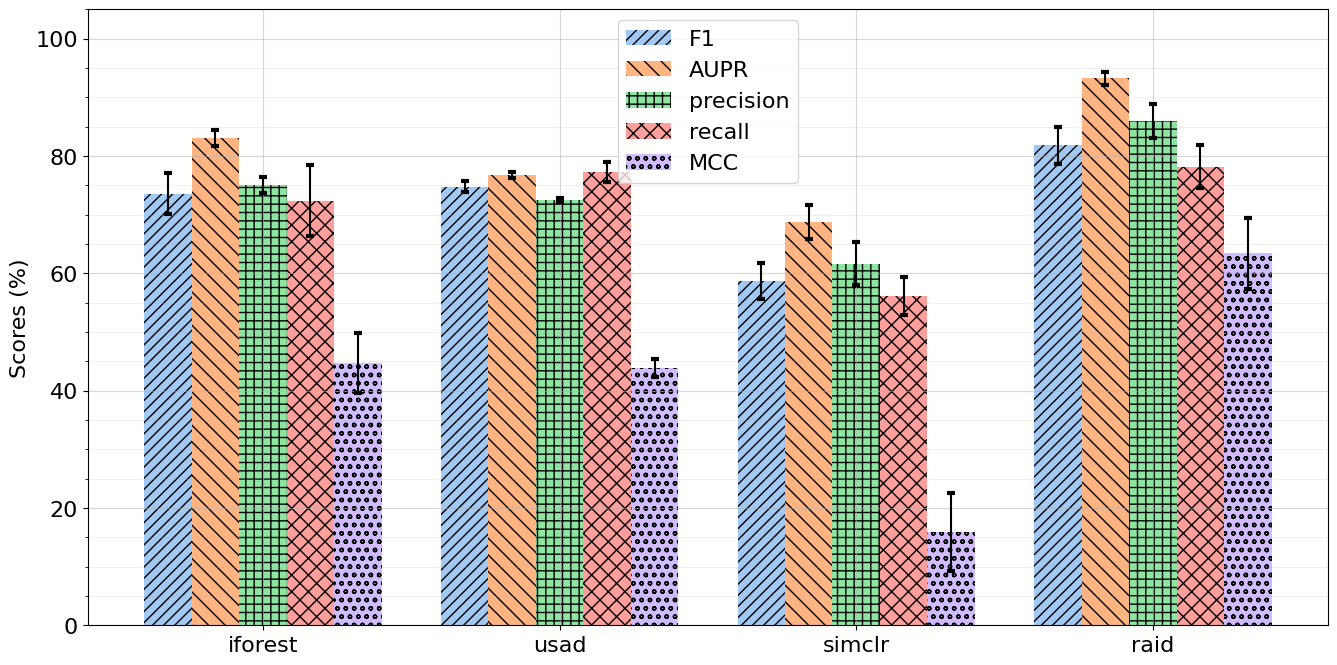
\includegraphics[width=.9\linewidth]{imgs/chapter_6/ad.png}
    \caption{Results of anomaly detectors of two-stage models.}
    \label{fig:chap_6:ad_results}
\end{figure*}


\subsubsection{Per-Class Performance Analysis}

Figures \ref{fig:chap_6:confusion_matrix} and \ref{fig:chap_6:per_class} provide a detailed comparison of the per-class performance metrics for T-Loss and RAID. Our approach demonstrates a significant advantage in efficiently distinguishing normal scenarios from both coverage and interference scenarios.

For normal scenarios, our solution achieves a notably lower misclassification rate compared to T-Loss, with 1,761 correctly classified normal samples versus 1,350 for T-Loss. This represents a substantial improvement in detecting normal behavior. Additionally, our solution attains perfect classification for interference scenarios, with a recall of 100\%, highlighting its robustness in detecting distinct anomaly patterns such as interference.

However, Fig. \ref{fig:chap_6:per_class} also reveals the limitations of our solution. It struggles to discriminate coverage scenarios, with a considerable number of coverage windows misclassified as normal. This indicates challenges in capturing the subtle variations and transitional patterns between normal and coverage states. In contrast, T-Loss, while less accurate overall, shows a more balanced performance in handling coverage scenarios. 

This trade-off underscores the strengths and weaknesses of our model: it is highly effective in detecting clear-cut anomalies but requires further refinement to enhance its sensitivity to nuanced variations between normal and coverage states. Future work could focus on addressing this limitation by incorporating advanced feature extraction techniques or domain-specific data augmentation strategies.


\takeaway{RAID model demonstrates superior performance in root cause diagnosis for Cloud VR scenarios, achieving the highest performance compared to both one-stage and two-stage approaches. Its robust anomaly detection stage significantly enhances its effectiveness, outperforming other methods in detecting distinct patterns such as interference. However, the model struggles with subtle variations in coverage scenarios, suggesting room for improvement in handling nuanced transitions.}

\begin{figure*}[!t]
  \centering
  \begin{tabular}{ c @{\hspace{0pt}} c}
  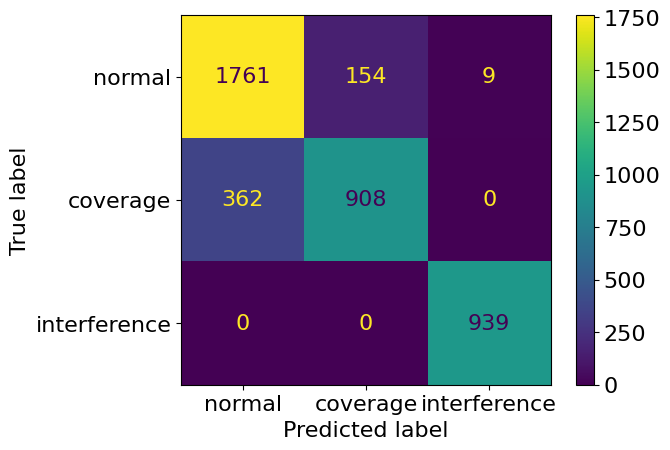
\includegraphics[width=0.5\textwidth]{imgs/chapter_6/cm_cats.png}
    &
  %\medskip
    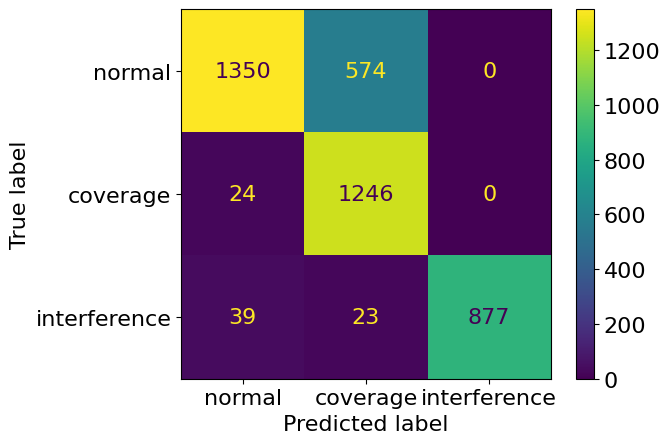
\includegraphics[width=0.5\textwidth]{imgs/chapter_6/cm_triplet.png}\\
     \small \textbf{(a) RAID} &
    \small \textbf{(b) T-Loss}  \\
  \end{tabular}
  \medskip
  \caption{Confusion matrix}
  \label{fig:chap_6:confusion_matrix}
\end{figure*}

\begin{figure*}[!t]
  \centering
  \begin{tabular}{ c @{\hspace{0pt}} c}
  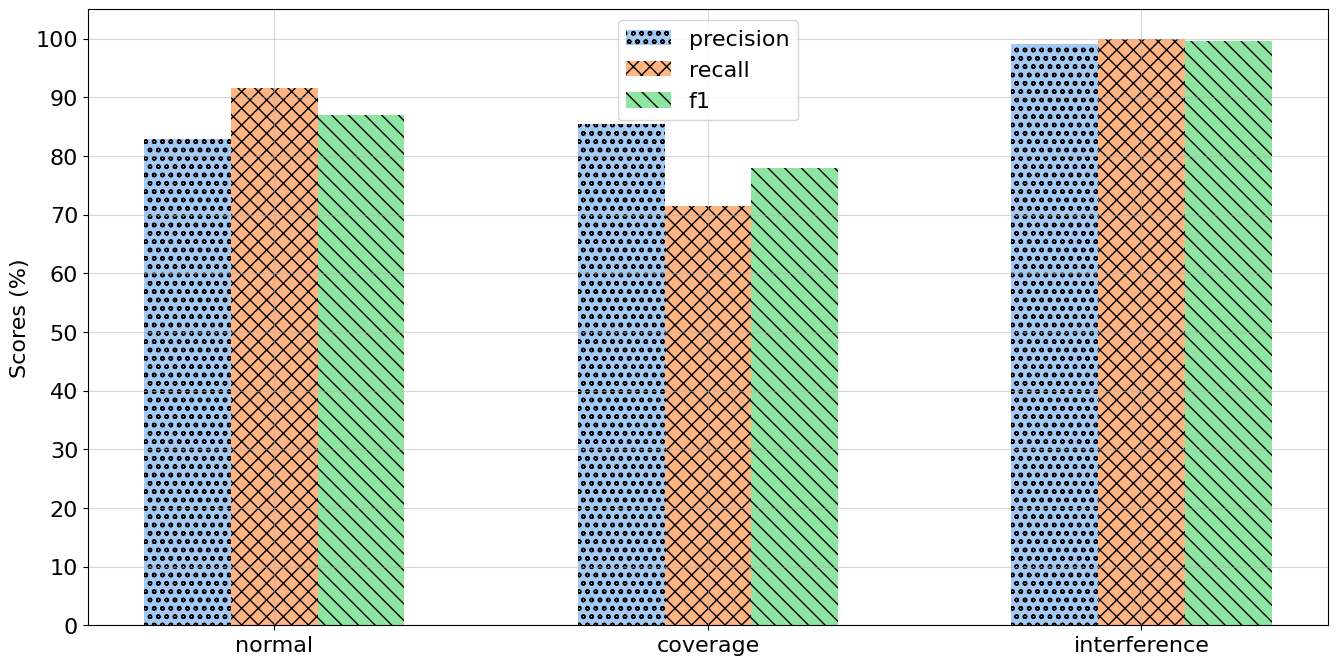
\includegraphics[width=0.5\textwidth]{imgs/chapter_6/per_class_cats.png}
    &
  %\medskip
    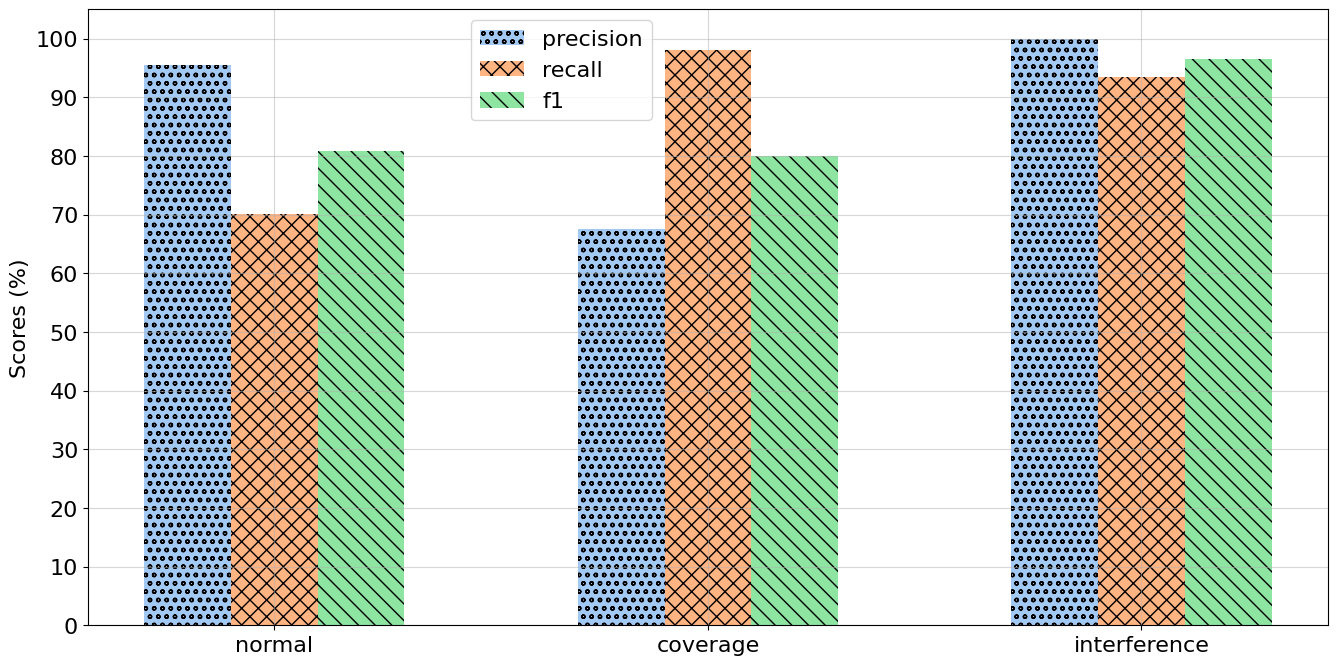
\includegraphics[width=0.5\textwidth]{imgs/chapter_6/per_class_triplet.png}\\
     \small \textbf{(a) RAID} &
    \small \textbf{(b) T-Loss}  \\
  \end{tabular}
  \medskip
  \caption{Per-class precision, recall and F1-score.}
  \label{fig:chap_6:per_class}
\end{figure*}


\subsection{Efficiency with Few Labels}

Fig. \ref{fig:chap_6:finetune_labels} illustrates the evolution of model performance as the percentage of labeled data increases. The left subplot depicts the accuracy scores across various label ratios, while the right subplot presents the corresponding F1-scores.

At the lowest label ratios (1\%-5\%), most models exhibit limited performance, reflecting the inherent difficulty of accurate root cause diagnosis (RCD) with minimal supervision. However, T-Loss and RAID stand out by achieving relatively higher accuracy and F1 scores, showcasing their ability to generalize effectively even with sparse labeled data. T-Loss benefits significantly from its triplet-based pretraining strategy, which efficiently captures meaningful representations from the unlabeled dataset, thereby enhancing fine-tuning performance. Similarly, the pretraining stage of RAID contributes to its robustness in low-label scenarios by effectively leveraging the anomaly detection process to prioritize relevant patterns.

As the label ratio increases, all models demonstrate steady improvement in performance, highlighting the benefits of additional labeled data. Notably, RAID and T-Loss consistently lead in performance, with our solution exhibiting a steady performance boost. This consistency underscores the robustness of RAID across varying levels of supervision. While T-Loss initially competes closely, its performance shows a slight decline between the 5\% and 20\% label ratios, coupled with increased variability, indicating potential sensitivity to the quality or distribution of labeled data in these ranges.

The findings from Fig. \ref{fig:chap_6:finetune_labels} highlight the efficiency of RAID in leveraging limited labeled data, making it an ideal solution for real-world scenarios where labeling is both expensive and time-consuming. Its performance with sparse labels, along with its stable scalability as more labeled data becomes available, firmly establishes RAID as the most suitable model in this evaluation.

\takeaway{RAID also demonstrates strong performance in scenarios with limited labeled data thanks to its anomaly detection stage that effectively prioritize relevant patterns. While T-Loss competes closely in low-label scenarios, its performance exhibits greater variability as label ratios increase.}

\begin{figure*}[!ht]
    \centering
    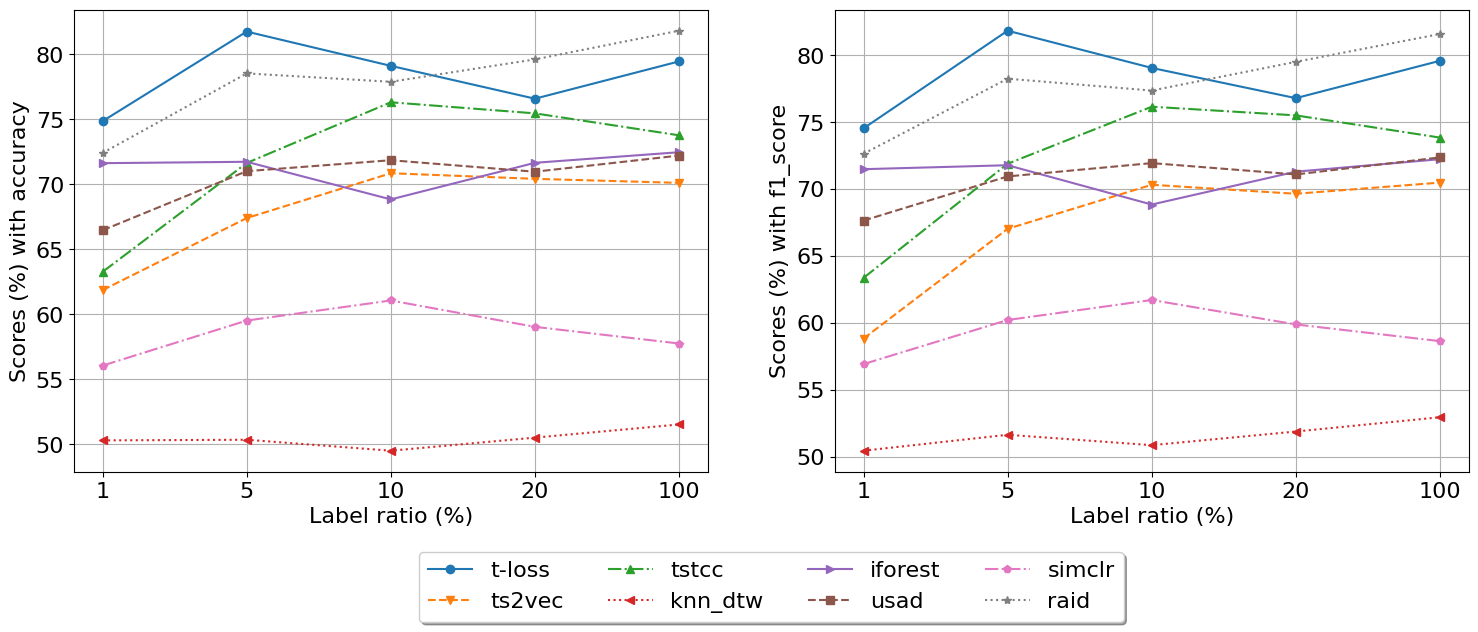
\includegraphics[width=\linewidth]{imgs/chapter_6/labels.png}
    \caption{Performance variation regarding the labels ratio.}
    \label{fig:chap_6:finetune_labels}
\end{figure*}

% On the contrary, models like TS-TCC and SimCLR show significant struggles in this low-label regime, as their reliance on large amounts of labeled data limits their capacity to achieve competitive performance. Similarly, one-stage methods such as T-Loss and TS2Vec exhibit modest improvements but fail to match the performance of two-stage approaches like CATS, which leverage a preliminary anomaly detection stage to guide fine-tuning.

\subsection{Time complexity}

Fig. \ref{fig:chap_6:time_complexity} presents the training time (in seconds) and inference time per time series (in milliseconds) for each of the RCD models. The model with the longest training time is Triplet, which takes approximately 300 seconds, while the fastest training model is 1-NN-DTW, completing training in 500 milliseconds. In terms of inference time, 1-NN-DTW significantly outpaces other models, with the highest inference time of 1800 milliseconds. In contrast, models such as Triplet or TS-TCC, achieve inference times as low as 0.5 milliseconds.

Our proposed solution, RAID, demonstrates a moderate training time of 200 seconds and an inference time of 3.5 milliseconds. While this inference time is the second highest among the models compared, it is still well-suited for real-time deployment, especially in our testbed where data is collected at frequent intervals (e.g., every 3 seconds). This makes RAID an excellent choice for RCD, as it balances moderate training overhead with sufficiently low inference latency, allowing for continuous monitoring and fast anomaly detection. Additionally, being a two-stage model, RAID offers a key advantage: when new causes or anomalies are detected, only the supervised classifier requires retraining. Most of the training time originates from the initial anomaly detection phase, unlike one-stage models that require complete retraining, including the pretraining phase. This makes RAID more efficient for scenarios requiring periodic updates or retraining, reducing overall downtime and resource consumption.

In summary, RAID strikes a practical balance between training efficiency and inference speed, making it highly effective for real-time RCD in dynamic and large-scale network environments.


\takeaway{RAID achieves a practical balance between training efficiency and inference speed, with a training time of 200 seconds and an inference time of 3.5 milliseconds. RAID's two-stage design further enhances its practicality by requiring retraining only for the supervised classifier when new anomalies are detected, unlike one-stage models that necessitate full retraining.}

\begin{figure*}[!ht]
    \centering
    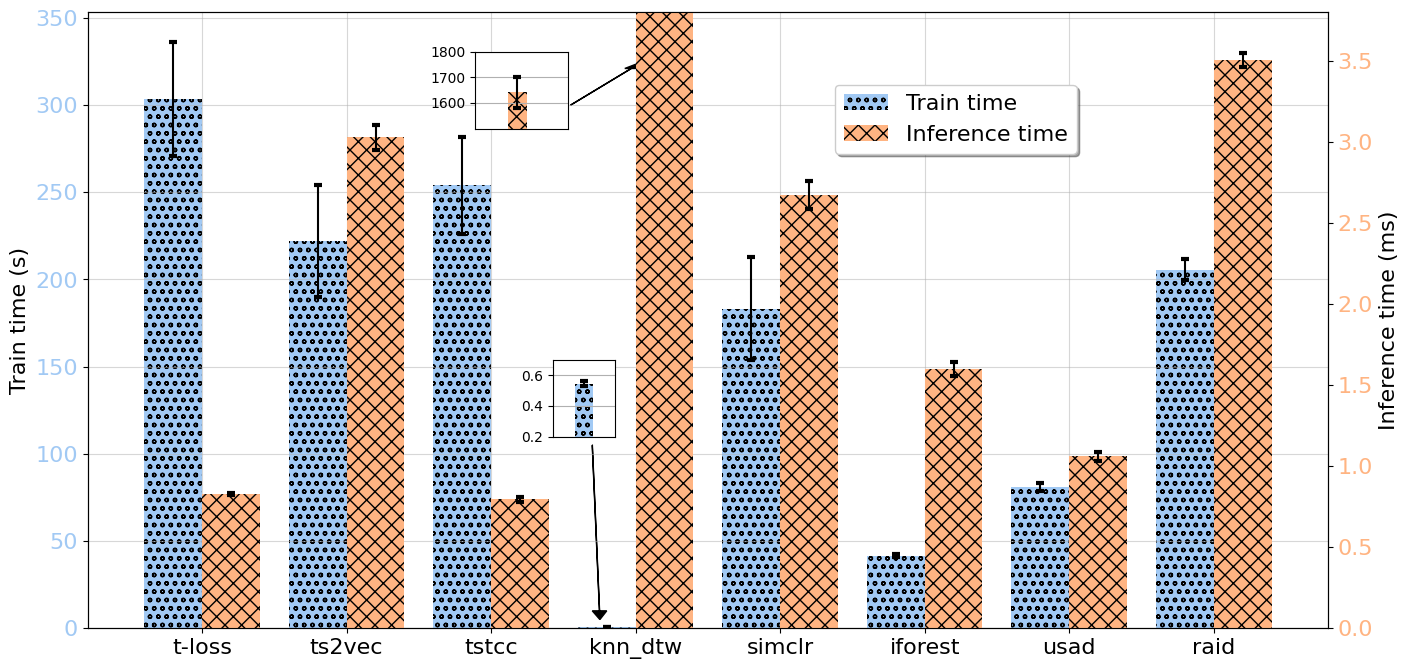
\includegraphics[width=\linewidth]{imgs/chapter_6/time.png}
    \caption{Time complexity of each model.}
    \label{fig:chap_6:time_complexity}
\end{figure*}